%% TC adaptation: seven internal hypotheses are consolidated into four RQs.
%% Numeric evidence remains bound to its frozen hardware/workload/quality contract.

\subsection{Setup and Research Questions}\label{sec:eval:setup}

We evaluate five checkpoints from two revision-generative ASR families:
Qwen3-ASR 0.6B/1.7B and Whisper tiny/base/small.en. The main system runs use
two RTX~3090 GPUs. The matched comparison uses the same 16 bilingual 30-s
sessions (c16; 480\,s of audio), whereas cross-family production results retain
their original family-specific workloads and references. Scale-out is measured
separately on one RHEL~7.6 node with eight 32-GB Tesla V100 PCIe GPUs and the
Transformers-eager backend. Quality is evaluated against an independent
canonical replay for Qwen and unprotected feedback for Whisper. We never pool
results across hardware, families, authority paths, or quality estimands.

\emph{Metrics and timing.} Audio xRT is completed audio seconds divided by
service wall time. Wall speedup divides singleton-reference wall time by
service wall time; GPU-normalized speedup additionally divides by the
service-to-reference GPU-count ratio (two for the RTX~3090 cells). Energy is
trapezoidally integrated from NVIDIA Management Library (NVML) power samples
and normalized by completed
audio seconds. Display latency measures ready-to-proposal completion, whereas
state/segment-commit latency measures ready-to-authorized installation; the two
clocks are never interchanged. Timed cells use immutable causal arrival
schedules, while wall and energy meters record real execution. The matched
Qwen cells use 2-s fine revisions and 6-s authority segments
($\granratio=3$). ``16/16 pass'' means that every Whisper production cell met
its frozen thresholds: wall speedup $\ge2.5\times$, GPU-normalized speedup
$\ge1.25\times$, energy reduction $\ge20\%$, display P99 $\le1.9$,s, commit
P99 $\le36$,s, audio amplification $\le1.2\times$, and zero semantic
violations.

The evaluation asks: \emph{RQ1}, does the feedback edge causally propagate a
local execution difference? \emph{RQ2}, does DGFT preserve transaction
integrity? \emph{RQ3}, what performance--quality--energy frontier does the
authority split expose, including against the nearest adapted baselines?
\emph{RQ4}, how does independent proposer/authority replication scale?

\subsection{RQ1: Causal Propagation}\label{sec:eval:rq1}

We enumerate 21 legal Whisper state pairs and apply the same isolated
batch-created divergence with the feedback edge present and removed, while
holding future inputs, batch assignments, and arithmetic realization fixed.
With feedback, 8/21 pairs propagate; without feedback, 0/21 do. Six pairs
remain divergent into the measured tail, where the revision amplification
factor (Definition~\ref{def:raf}) reaches 153. This intervention identifies
feedback as the propagation channel; it does not estimate a production
prevalence.

\subsection{RQ2: Transaction Integrity}\label{sec:eval:rq2}

We validate every accepted install in 800 Qwen events (480 SG and 320 DGFT)
and 1{,}048 Whisper commits. Under the trust and binding assumptions of
Section~\ref{sec:dgft}, all completed sessions have monotone terminal frontiers,
with zero observed transaction-install, output/state, stale-result, or replay
violations. No stale install was attempted in these production traces; hence
they validate accepted-history integrity rather than fault-injected stale
rejection.

A deterministic state-machine fuzzer supplies the adversarial complement. It
issues 250{,}000 attempts across 64 sessions and 24 invalid/replay classes,
including cross-session and cross-epoch substitution, certificate tampering,
stale parents, frontier gaps/overlaps, duplicates, and replays. The runtime
accepts all 10{,}000 valid commits and rejects all 240{,}000 mutations, with no
invariant violation. This is exhaustive validation over the evaluated traces
and mutation suite, not a zero-failure-probability claim; it excludes Byzantine
trusted components, GPU worker crashes, and wall-clock expiry.

To isolate transaction logic from accelerator execution, we benchmark the
production commit primitive on the submission host using 31 randomized
repeats of 20{,}000 valid calls (2{,}000-call warmup; 256-token prompt,
32-token display, and eight speculative descendants). The median full commit
is 101.107\,$\mu$s versus 19.077\,$\mu$s for the same immutable-state
materialization without checks, a paired incremental cost of
81.960\,$\mu$s/commit; the full-commit P99 across repeat aggregates is
104.514\,$\mu$s. This host-side protocol microbenchmark is not GPU or
end-to-end speedup evidence; Supplementary Section~S4 gives all variants and
the existing online critical-section cross-check.

\subsection{RQ3: Service Frontier, Quality, and Baselines}
\label{sec:eval:rq3}

\paragraph{Matched authority configurations}
Figure~\ref{fig:ablation} compares complete configurations on the identical c16
workload: SG ($\granratio=1$, FP16 singleton authority), Coarse-DGFT
($\granratio=3$, FP32 batched authority), and Hybrid-DGFT
($\granratio=3$ plus selective replay). Authority precision, execution mode,
and granularity change together, so this is not a precision-independent
ablation of $\granratio$.

\begin{figure}[t]
  \centering
  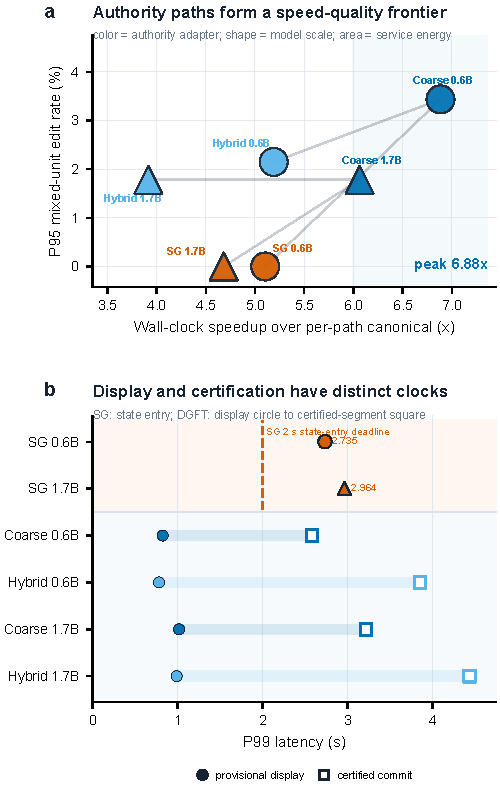
\includegraphics[width=\columnwidth]{figures/f3_authority_frontier_column.pdf}
  \caption{Matched c16 authority configurations. Marker area denotes energy;
  display and certified-commit latencies remain distinct estimands.}
  \label{fig:ablation}
\end{figure}

Coarse reduces service wall time from 14.905 to 10.759\,s (0.6B) and from
16.285 to 12.763\,s (1.7B), giving direct throughput gains of
$1.39\times$ and $1.28\times$ over SG. Its separately normalized headline
speedups are $6.88\times/6.06\times$ over each path's frozen all-singleton
reference; these normalizations are not divided to obtain the matched ratios.
SG's synchronized terminal burst yields certified state-entry P99
2.735/2.964\,s and 2-s miss rates 3.33\%/4.17\%. Coarse/Hybrid instead expose
display P99 $\le1.018$\,s and segment-commit P99 2.582--4.437\,s. Coarse energy
relative to SG changes from $-4.4\%$ on 0.6B to $+15.1\%$ on 1.7B; Hybrid costs
$+16.8\%/+54.2\%$. The reversal confirms that the complete authority path,
not granularity alone, determines the operating point.

\paragraph{Cross-family production and quality}
On Qwen, Coarse-DGFT reaches $6.88\times/6.06\times$ wall speedup,
$3.44\times/3.03\times$ GPU-normalized speedup, and 59.8\%/51.0\% energy
reduction for 0.6B/1.7B. On Whisper, the same transaction runtime passes all
16 production cells: median wall speedup is $2.841\times$ (range
2.633--3.849), GPU-normalized speedup is $1.421\times$, median energy reduction
is 31.13\%, and display P99 is at most 1.492\,s. Figure~\ref{fig:production}
reports each family against its own baseline; the magnitudes are not compared
across columns.

\begin{figure*}[t]
  \centering
  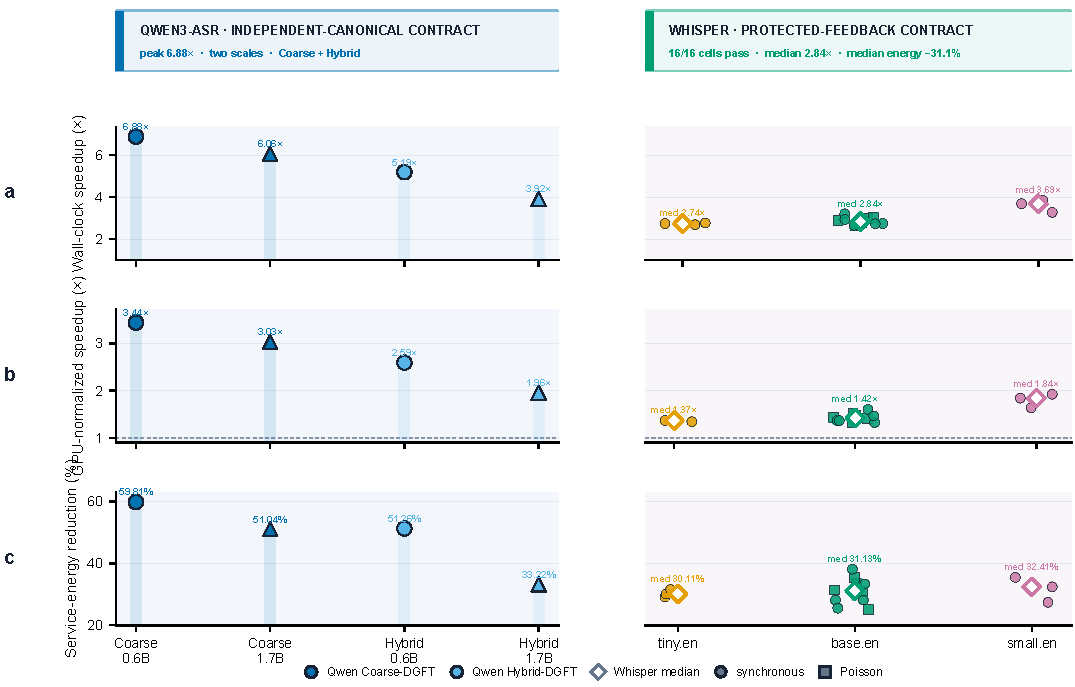
\includegraphics[width=\textwidth]{figures/f4_production.pdf}
  \caption{Production performance under family-specific contracts. Qwen and
  Whisper use different baselines and are not pooled.}
  \label{fig:production}
\end{figure*}

Qwen's mixed-unit edit rate against independent FP16 singleton replay has
empirical P95 $\le3.43\%$ (worst session 5.41\%; no catastrophic case). On
deterministic 64-utterance holdouts from \emph{LibriSpeech test-clean} and
\emph{AISHELL-1}, respectively, 0.6B/1.7B obtain English WER
2.15\%/2.30\% and Chinese CER 2.71\%/2.16\%, with 256/256 terminal outputs
exactly matching singleton authority and partial-revision edit rates
24.7--31.8\%. These are fixed holdouts, not full-corpus leaderboard results.

For Whisper, protection improves WER relative to unprotected feedback for
tiny/base/small.en by $-12.23/-18.21/-25.27$ points on development sessions
and $-8.26/-11.03/-13.76$ on the untouched cohort. All one-sided 95\%
bootstrap upper bounds remain below zero. The untouched cohort contains 40
long sessions per model, deterministically assembled from 214 previously
unused source utterances; the long session is the bootstrap unit. These
family-specific quality questions remain separate (Figure~\ref{fig:quality}).

\begin{figure}[t]
  \centering
  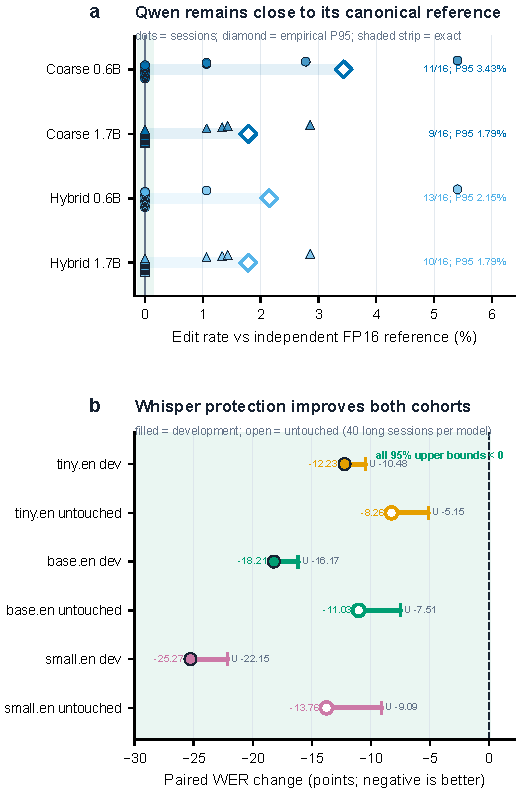
\includegraphics[width=\columnwidth]{figures/f5_quality_column.pdf}
  \caption{Family-specific quality. Qwen measures edit distance to an
  independent canonical replay; Whisper measures paired WER change from
  unprotected feedback.}
  \label{fig:quality}
\end{figure}

\paragraph{Nearest adapted baselines}
Table~\ref{tab:normal-adaptations} compares all methods on the independent
V100 c16 workload; all 240 display events per cell meet the 2-s display SLO.
Against an LLM-42-style revision adaptation that verifies every revision,
Coarse-DGFT improves audio throughput by $6.91\times/5.64\times$ on
0.6B/1.7B. Against MarginGate-inspired scheduling, Coarse is 5.6\% slower on
0.6B and 11.5\% faster on 1.7B. The latter has no state-write authorization
contract, so this comparison quantifies normal-load cost rather than equivalent
safety.

\tbl{t8_normal_slo_adaptations}

On a separate overloaded c32 stress trace, MarginGate-inspired verification
checks 3.02\% of events but misses the known state-changing flip; an
owner/version-only fence also accepts it. Always-verifying LLM-42-style replay
removes the error at 1.565 events/s, whereas RevTrace verifies 5.05\%, removes
the error, and reaches 3.046 events/s ($1.95\times$). Because P99 is
6.107\,s, this trace measures safety cost, not serving capacity. A legal
execution-shape suite (batch size, slot, composition, and repeat) induces
1{,}021 proposal--canonical mismatches among 1{,}848 target-row evaluations;
the frozen risk scheduler has zero observed false-safe events. Risk schedules
verification but never certifies a write~\cite{chu2026margingate,zhang2026llm42}.

\subsection{RQ4: Replica Scaling and Capacity}\label{sec:eval:rq4}

The independent V100 study contains 84 cells spanning authority
microprofiles, c16 baselines, c16--c128 replica allocations, and
$\granratio\in\{1,3,5\}$ attribution. We freeze the headline allocations and
repeat 30 additional cells (three runs per model and configuration); ranges in
Figure~\ref{fig:v100-dual-plane} are min--max. Repeated batched executions
agree, but each model still has 62 batch--singleton request mismatches across
precisions and batch sizes. FP32 batching is therefore a contract-scoped
authority, not an unconditional singleton-equivalence certificate.

At c16, SG/Hybrid/Coarse reach $4.682/5.764/6.072\times$ wall speedup on
0.6B and $3.248/4.657/4.893\times$ on 1.7B. Balanced four-proposer plus
four-authority replication at c64 sustains median $157.786\times/111.722\times$
audio real-time throughput. Display P99 is 1.089/1.394\,s with zero misses
over 2{,}880 repeated events per model; certified-segment commit P99 is
separately 3.080/4.890\,s. At c128, display P99 rises to 2.079/2.730\,s and
commit P99 to 6.012/10.153\,s, while throughput saturates. Thus c64 is the
largest measured point satisfying the display SLO for both models, and c128 is
retained as the failed boundary.

An authority-heavy 3+5 allocation at c64 lowers the authority/proposer service
ratio but also lowers throughput to $93.788\times/77.704\times$ and yields
display P99 1.756/2.209\,s; adding authority replicas does not repair the
proposer bottleneck, and balanced 4+4 dominates. At
$\granratio=1$, FP32 authority/proposer ratios 2.216/2.669 reduce throughput to
$18.603\times/12.294\times$; at $\granratio=5$, the ratios fall below one and
throughput recovers to $40.630\times/33.909\times$. These results support the
two-stage cost model: balanced replication expands capacity, while coarse
authority becomes economical only after sufficient amortization. They
establish single-node, not multi-node, scaling.

\begin{figure*}[t]
  \centering
  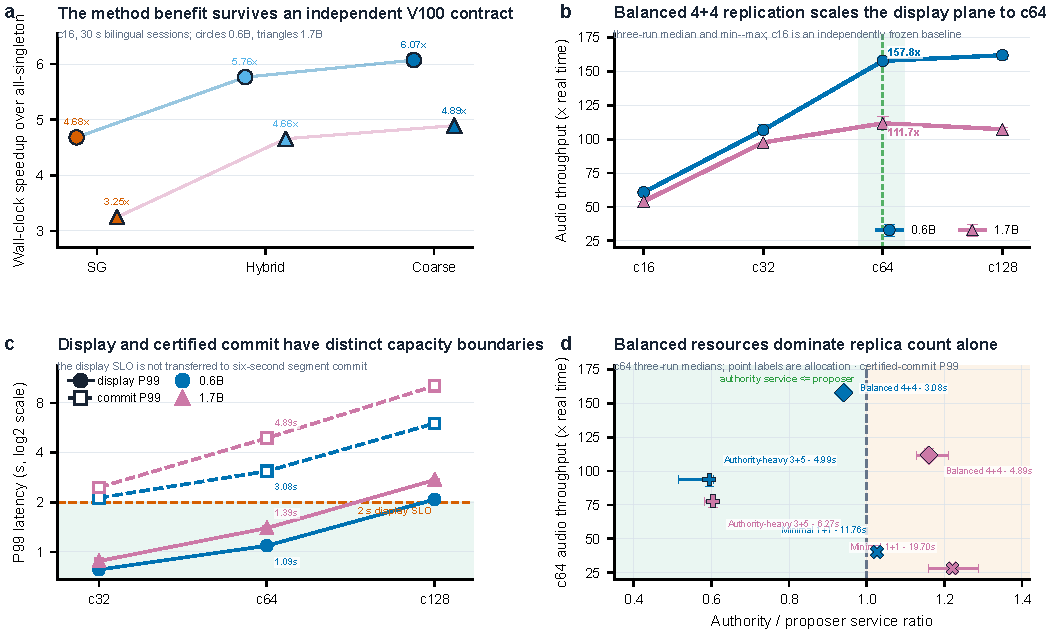
\includegraphics[width=\textwidth]{figures/f7_v100_dual_plane.pdf}
  \caption{Independent V100 replica scaling. Balanced 4+4 reaches the c64
  display-SLO boundary; display and certified-commit latency are reported on
  distinct clocks. Points at c32--c128 show three-run medians and min--max
  ranges.}
  \label{fig:v100-dual-plane}
\end{figure*}
